\documentclass{hwset}

\name{Erich L Foster}
\class{Calculus I}
\duedate{20 April 2011}
\assignment{Homework 11}

\begin{document}
\begin{problem}[1.]
	Prove the following  equations have exactly one real solution in the given
	interval (do not find the root)
	\begin{enumerate}
		\item $\cos x = e^x$ in the interval $[-1,1]$.
		\item $\ln x = \tan x$ in the interval $(3,4.5)$
	\end{enumerate}
\end{problem}

\begin{enumerate}
	\item \begin{solution} \tbf{Proof:}
		Let $f(x) = \cos x - e^x$ then since both $e^x$ and $\cos x$ are continuous
		and differential on the given interval then so is $f(x)$. Since $f(x)$ is
		continuous on $[-1,1]$ by the IVT we know that $f(x)$ achieves every value
		between $f(-1)\approx 0.17$ and $f(1)\approx -2.2$. Since zero is between
		$f(-1)$ and $f(1)$ there must be at least one zero in the interval $[-1,1]$.
		\\
		On the other hand, assume that $f(x) = 0$ for two values of $x\in [-1,1]$,
		i.e. $f(x_1) = f(x_2) = 0$ for $x_1,x_2\in [-1,1]$. Since $f(x)$ is
		continuous on $[-1,1]$ and differential on $(-1,1)$ and $f(x_1) = f(x_2)$ we
		know, by Rolle's Theorem, that there exists a $c\in (-1,1)$ such hat $f'(c)
		= 0$. However,
		\begin{equation*}
			f'(x) = \sin x - e^x < 0\; \forall x\in(-1,1).
		\end{equation*}
		a contradiction and so our initial assumption must have been
		incorrect. Therefore, we must have exactly one root to $f(x)$ in the
		interval $[-1,1]$, which implies $e^x = \cos x$ for exactly one $x\in
		[-1,1]$. 
	\end{solution}
	\item \begin{solution} \tbf{Proof:}
		Let $f(x) = \ln x - \tan x$ then since both $\ln x$ and $\tan x$ are continuous
		and differential on the given interval then so is $f(x)$. Since $f(x)$ is
		continuous on $[3,4.5]$ by the IVT we know that $f(x)$ achieves every value
		between $f(3)\approx 1.24$ and $f(4.5)\approx -3.13$. Since zero is between
		$f(3)$ and $f(4.5)$ there must be at least one zero in the interval $[3,4.5]$.
		\\
		On the other hand, assume that $f(x) = 0$ for two values of $x\in [3,4.5]$,
		i.e. $f(x_1) = f(x_2) = 0$ for $x_1,x_2\in [3,4.5]$. Since $f(x)$ is
		continuous on $[3,4.5]$ and differential on $(3,4.5)$ and $f(x_1) = f(x_2)$ we
		know, by Rolle's Theorem, that there exists a $c\in (3,4.5)$ such hat $f'(c)
		= 0$. However,
		\begin{equation*}
			f'(x) = \frac{1}{x} - \sec^2 x < 0\; \forall x\in(3,4.5).
		\end{equation*}
		a contradiction and so our initial assumption must have been
		incorrect. Therefore, we must have exactly one root to $f(x)$ in the
		interval $[-1,1]$, which implies $\tan x = \ln x$ for exactly one $x\in
		[3,4.5]$. 
	\end{solution}
\end{enumerate}

\begin{problem}[2.]
	Given $f(x) = \sin 2x $ in $[0, \sfrac{\pi}{2}]$
	\begin{enumerate}
		\item Verify $f$ meets the conditions of the Mean Value Theorem.
		\item Find the value(s) of $c$ that satisfies the conclusion of the Mean
			Value Theorem.
	\end{enumerate}
\end{problem}

\begin{enumerate}
	\item \begin{solution}
		Since $\sin x$ is continuous and differential on $(-\infty,\infty)$ then so
		is $\sin 2x$ and therefore $\sin 2x$ is continous on $[0,\sfrac{\pi}{2}]$
		and differential on $(0,\sfrac{\pi}{2}$.
	\end{solution}
	\item \begin{solution}
		Since $f(x)$ satisfies the hypotheses of the MVT there exists a $c\in
		(0,\sfrac{\pi}{2}$ such that 
		\begin{align*}
			f'(c) &= \dfrac{f(\sfrac{\pi}{2}) - f(0)}{\sfrac{\pi}{2} - 0} \\
			2\cdot \cos 2c &= 0 \\
			c &= \frac{\cos^{-1} 0}{2} \\
			c &= \boxed{\frac{\pi}{4}.}
		\end{align*}
	\end{solution}
\end{enumerate}

\begin{problem}[3.]
	For $f(x) = \left| x^3 + 1\right|$ defined on the entire real	number line
	\begin{enumerate}
		\item Find all Critical Points
		\item Find all Inflection Points
		\item Use the First Derivative to find any max/mins.
		\item Use the Second Derivative to find any max/mins.
	\end{enumerate}
\end{problem}

\begin{enumerate}
	\item \begin{solution}
		To find all critical points we must determine when the derivative is zero
		and determine where the derivative is undefined. First let's find where the
		derivative is undefined since this will also be required for determining the
		derivative. The derivative will be undefined when $f(x)=x^3+1=0$, i.e.
		$x=-1$ since there will be a sharp corner at this point. The function $f(x)$
		can therefore be written as
		\begin{equation*}
			f(x) = \begin{cases}
				x^3+1 & x \ge -1\\
				-x^3 - 1 &  x < -1
		\end{cases}
		\end{equation*}
		Thus the derivative is 
		\begin{equation*}
			f'(x) = \begin{cases}
				3x^2 & x > -1\\
				-3x^2 & x < -1
			\end{cases}
		\end{equation*}
		From this we see that the critical points are $x=\{-1,0\}$.
	\end{solution}
	\item \begin{solution}
		To find inflection points we must determine where $f''(x) = 0$ and where
    $f''(x)$ is undefined.
		\begin{equation*}
			f''(x) = \begin{cases}
				6x & x > -1\\
				-6x & x < -1
			\end{cases}
		\end{equation*}
		From this we see that $f''(x) = 0$ when $x=0$ and $f''(x)$ is undefined when
    $x=-1$. However, we must check that $f''(x)$ actually changes sign at $x=0$.
    Since it changes from negative to positive as we travel from right to left
    across $x=0$ there is indeed an inflection point when $x=0$. On the other
    hand when we travel from left to right across $x=-1$ we see the value of
    $f''(x)$ go from positive to negative and so $x=-1$ would also be an
    inflection point.
  \end{solution}
	\item \begin{solution}
		Using the first derivative
	\begin{center}
	\begin{tikzpicture}
		\draw[<->] (0,0) node[above,fill=none] {$f'(x)$} 
		-- (1.5,0) node[above,fill=none] {$(-)$} 
		-- (4,0) node[above,fill=none] {$(+)$} 
		-- (6.5,0) node[above,fill=none] {$(+)$} 
		-- (8,0) node[right,fill=none] {$x$};
		\draw (3,0.1) -- (3,-0.1) node[below,fill=none] {$-1$};
		\draw (5,0.1) -- (5,-0.1) node[below,fill=none] {$0$};
	\end{tikzpicture}
	\end{center}
		we see that $f(-1) = 0$ is a minimum and $f(0) = 1$ is a saddle-point.
	\end{solution}
	\item \begin{solution}
		The Second derivative tells us nothing at $x=-1$ since it is undefined
		there. However, since $f''(0)=0$ we see that the point $(0,1)$ is a saddle-point.
	\end{solution}
\end{enumerate}

\begin{problem}[4.]
	Graph $f(x) = \dfrac{4x}{x^2 + 1}$. Don't use a table of values and show all
	work.
\end{problem}

\begin{solution}
	To draw the graph we first find all critical points.
	\begin{align*}
		f'(x) &= 4(x^2+1)^{-1} - 8x^2(x^2+1)^{-2} = 0 \\
		\Rightarrow& 4(x^2+1) - 8x^2 = 0 \\
		x &= \pm 1 \\
	\end{align*}
	and $f'(x)$ is undefined when
	\begin{equation*}
		x^2 + 1 = 0.
	\end{equation*}
	But, this doesn't have a solution for real numbers and therefore $f'(x)$ is
	always defined. Thus, our critical points are $x=\pm 1$. \\
	We also must determine when the function is increasing and decreasing, so
	let's use a number line of $f'(x)$
	\begin{center}
	\begin{tikzpicture}
		\draw[<->] (0,0) node[above,fill=none] {$f'(x)$} 
		-- (1.5,0) node[above,fill=none] {$(-)$} 
		-- (4.5,0) node[above,fill=none] {$(+)$} 
		-- (7.5,0) node[above,fill=none] {$(-)$} 
		-- (9,0) node[right,fill=none] {$x$};
		\draw (3,0.1) -- (3,-0.1) node[below,fill=none] {$-1$};
		\draw (6,0.1) -- (6,-0.1) node[below,fill=none] {$1$};
	\end{tikzpicture}
	\end{center}
	Thus, $f(x)$ is increasing when $x\in [-1, 1]$ and $f(x)$ is decreasing when
	$x \in \left(-\infty, -1\left]\, \bigcup\, \right[1, \infty\right)$.
	Now, we must find the inflection points.
	\begin{align*}
		f''(x) &= -8x(x^2+1)^{-2} - 16x(x^2+1)^{-2} + 16x^3(x^2+1)^{-3} = 0 \\
		\Rightarrow& -8x(x^2+1) - 16x(x^2+1) + 16x^3 = 0 \\ 
		&-x^3 - x - 2x^3 - 2x + 2x^3 = 0 \\ 
		&-x^3 - 3x = 0 \\ 
		&x = 0
	\end{align*}
	And therefore our inflection point is $x = 0$.
	Next, let's determine which critical points are min/max by using the second
	derivative test.
	\begin{equation*}
		f''(-1) = 4 \qquad f''(1) = -4
	\end{equation*}
	Thus, we see that $f(-1) = -2$ is a minimum and $f(1) = 2$ is a maximum. \\
	We also need to determine the concavity of our function. From when we used the
	second derivative test we see that $f''(x) < 0$ when $x<0$ and $f''(x)>0$ when
	$x>0$ and therefore $f(x)$ is concave up when $x>0$ and concave down
	when $x<0$.
	Finally, we must determine the behavior of $f(x)$ as $x\to \pm \infty$.
	\begin{equation*}
		\lim_{x\to \pm \infty} \dfrac{4x}{x^2+1} = \lim_{x\to \pm \infty}
		\dfrac{\sfrac{4}{x}}{1+\sfrac{1}{x^2}} = 0 
	\end{equation*}
	And the graph of $f(x)$ is 
	\begin{figure}[h]
	\begin{center}
	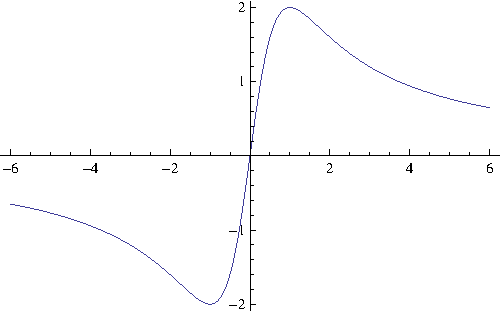
\includegraphics{HW11_4.pdf}
  \caption{Graph for Problem 4}
	\end{center}
	\end{figure}
\end{solution}

\begin{problem}[5.]
	Given $f$ is a continuous function and $f(0) = 0$ use the following table
	to graph the function $f$
	\begin{center}
	\begin{tikzpicture}
		\draw (-1,0) node[above,fill=none] {$x$} -- (0,0) node[above,fill=none]
		{$-\infty$} -- (2,0) node[above,fill=none] {$1$} -- (4,0)
		node[above, fill=none] {$4$} -- (6,0) node[above, fill=none]
		{$6$} -- (8,0) node[above, fill=none] {$+\infty$};
		\draw (-0.5,0.5) -- (-0.5,-0.75) node[left,fill=none] {$f'(x)$} --
		(-0.5,-2) node[above left,fill=none] {$f''(x)$};
		\draw[dashed] (2,0) -- (2,-2);
		\draw[dashed] (4,0) -- (4,-2);
		\draw[dashed] (6,0) -- (6,-2);
		\node at (0.5,-0.75) {$+$};
		\node at (3,-0.75) {$-$};
		\node at (5,-0.75) {$-$};
		\node at (7,-0.75) {$+$};
		\node at (0.5,-1.75) {$-$};
		\node at (3,-1.75) {$-$};
		\node at (5,-1.75) {$+$};
		\node at (7,-1.75) {$+$};
	\end{tikzpicture}
	\end{center}
\end{problem}

\begin{solution}
	The graph should have be shaped like the one below and should go through the
	point $(0,0)$.
	\begin{figure}[h]
	\begin{center}
	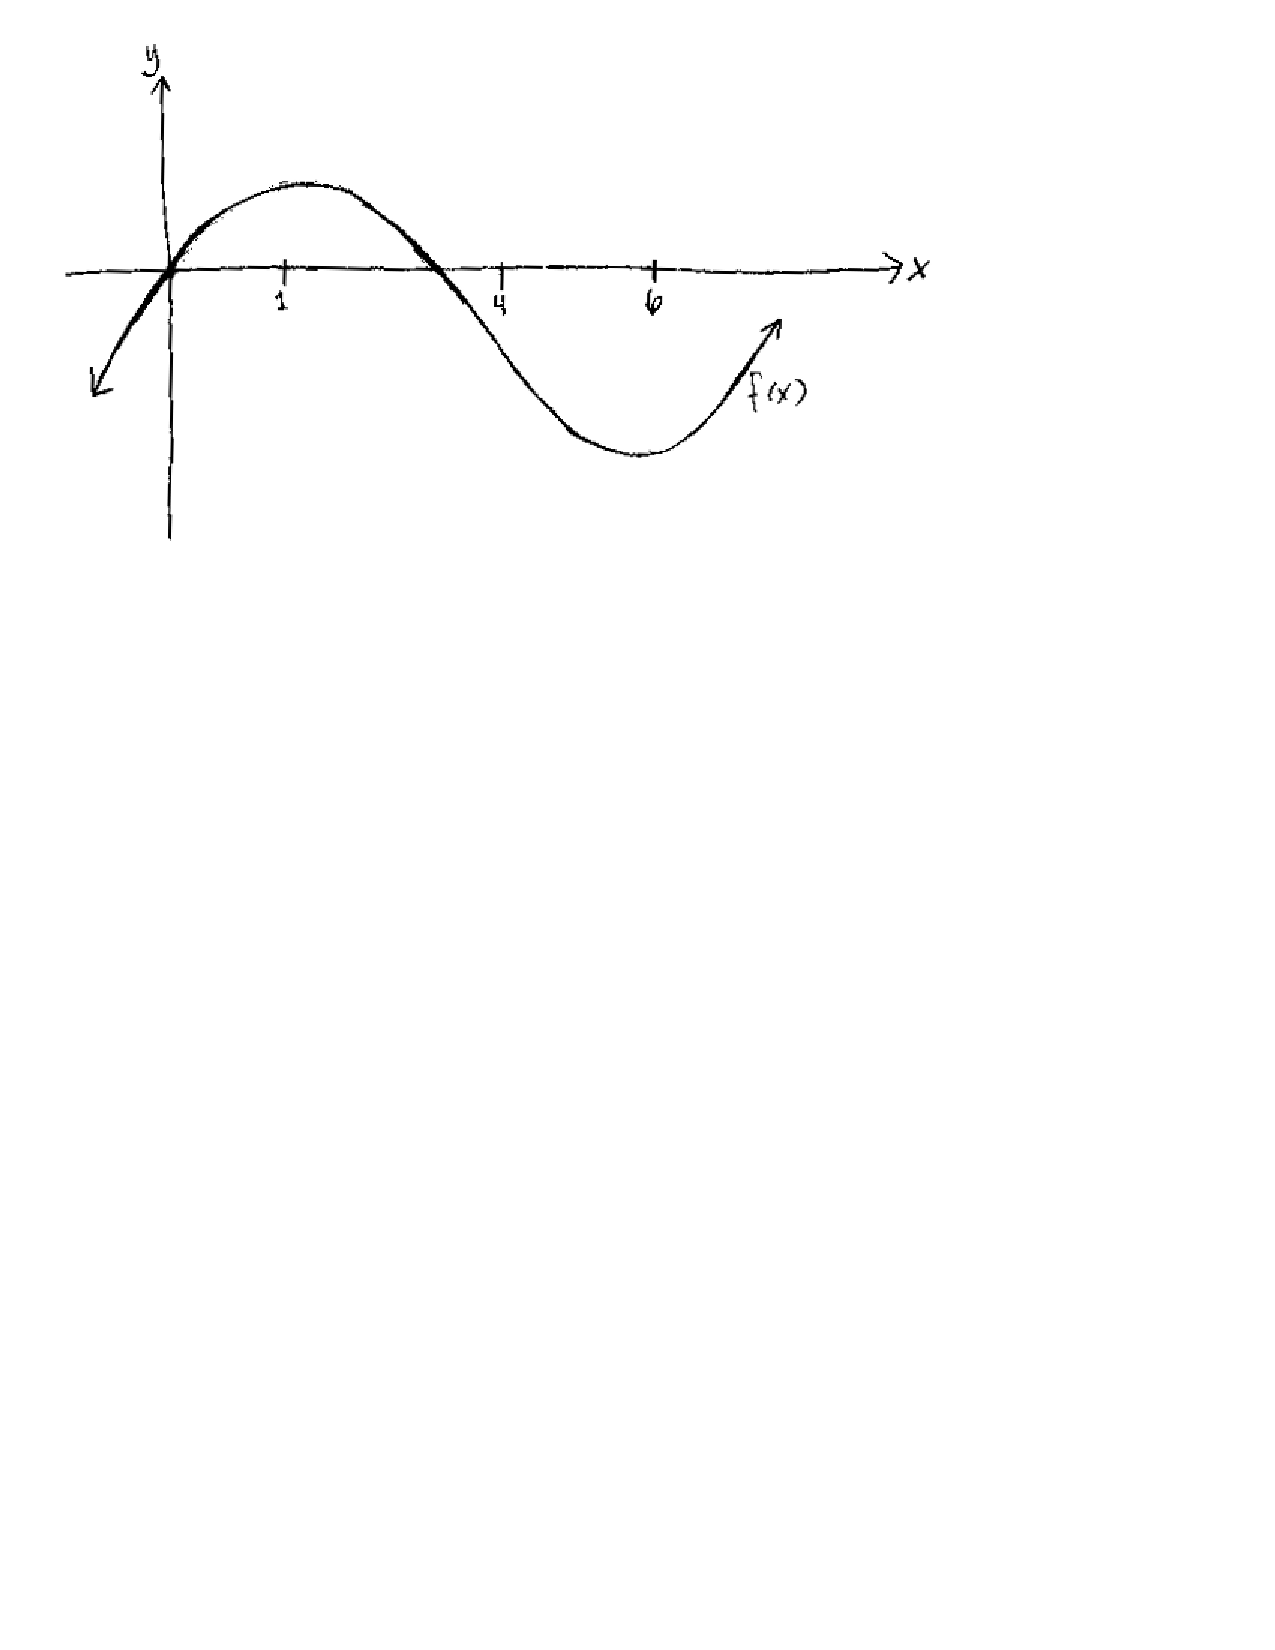
\includegraphics[trim=0.1 6.08in 1.59in 0.3in, clip]{HW11_5.pdf}
  \caption{Graph for Problem 5}
	\end{center}
	\end{figure}
\end{solution}

\end{document}
